\documentclass[11pt]{article}
\usepackage[utf8]{inputenc}
\usepackage[T1]{fontenc}
\usepackage{newtxtext} % Times New Roman
\usepackage[top=3cm, bottom=2cm, left=3cm, right=2cm]{geometry}
\usepackage{ragged2e}
\usepackage{enumitem}
\usepackage{setspace}
\usepackage{makeidx}
\usepackage{graphicx}
\usepackage{afterpage}
\usepackage{booktabs}
\usepackage{float}
\usepackage{caption}

\makeindex % Criar índice depois


% Início do corpo do texto
\begin{document}

\justifying % Texto justificado
\onehalfspacing % Espaçamento de 1,5 linha
\setlength{\parindent}{0cm}  % Indentação dos parágrafos
\renewcommand*\familydefault{\rmdefault}
%-----------------------------------------------------------%
% Capa                                
%-----------------------------------------------------------%
\thispagestyle{empty}
\begin{center}

\includegraphics[scale=0.6]{0-Capa/logo-dep.jpg}\\
\vspace*{.8cm}
{\huge \textbf{UNIVERSIDADE FEDERAL DE SÃO CARLOS}}\\
\vspace*{.8cm}
{\Large \textbf{SIMULAÇÃO DE SISTEMAS}}\\
\vspace*{3cm}
{\Large \textbf{Projeto para uma central de atendimentos}}\\
\vspace*{4.5cm}
\begin{flushright}
    \onehalfspacing
    {\Large  João Victor Pantaroto Neves - 769856}\\
    {\Large  João Vitor Carnaval Duarte - 800346}\\
    {\Large  Lucas C. Brandão da Silva - 758885}\\
    {\Large  Mariana Nakandakari  - 770107}\\
    {\Large  Pedro Peverari Di Lallo  - 792328}\\
    \vspace*{.3cm}
    {\Large \textbf{Professor:}}
    {\Large Rafael Ferro Munhoz Arantes }\\
\end{flushright}
\vspace*{\fill}
{\large \bf SÃO CARLOS / 2023}
\end{center}

\newpage{}
\tableofcontents{}
\newpage{}

\section{Introdução}

O setor de turismo apresenta grande potencial para otimização. Esse potencial deriva, sobretudo, do fato de que uma grande parte dessa indústria é baseada no estabelecimento de rotas. Dessa maneira, é possível aproximar, por exemplo, o planejamento de roteiros turísticos a problemas clássicos da pesquisa operacional, como o problema do caixeiro viajante e suas variações.

Nesse sentido, o “modelo” de problema com o qual mais se encaixa essa operação é o OPTW, ou “Problema de Orientação com Janelas de Tempo” (Gonçalves, V. A., et al, 2017) ou com coleta de prêmios. Entretanto, porque e em qual direção precisariam ser otimizadas rotas turísticas? Na máxima satisfação do cliente para um mínimo custo a ele. Para ilustrar o problema basta pensar em um caixeiro que visita atrações dentro de limites e intervalos de tempo, recebe um nível de satisfação em cada uma.

Outras interpretações possíveis para o problema são o PTPPP (Profitable Tour Problem with Priority Prizes), sugerido por Morabito (et al., 2014), como colocado por Silva  (et al, 2018). No entanto, ainda seria preciso considerar os horizonteis temporais caso essa seja a interpretação mais consistente do problema. Nesta situação, a ordem de visitação também importaria para os prêmios.

Algumas considerações, no entanto, são importantíssimas para a aplicação desse pensamento ao planejamento de roteiros turísticos. A primeira delas é que uma viagem raramente é planejada para apenas um dia. Esse comentário é especialmente verdadeiro para regiões com muitas atrações: imagine conhecer Roma, por exemplo, em apenas algumas horas. Não seria possível, e nem satisfatório ao turista.

A segunda é que, além de ter que retornar à um galpão, ou aeroporto, ou um ponto inicial semelhante, o turista precisa voltar à hotéis para que descanse. Dependendo a extensão do roteiro, porém, este hotel não é necessariamente sempre o mesmo, ao contrário do ponto inicial.

Outro ponto importante é que as atrações não podem ser visitadas em qualquer período do dia - alguns pontos turísticos podem só funcionar pela manhã, por exemplo. Além disso, é necessário que o viajante faça pausas para almoço e tenha horários livres. Quanto aos horários de almoço, vale salientar que os restaurantes certamente apresentarão restrições temporais, além de acrescentarem aos custos da rota. 

A representação completa do problema, então, é uma implementação multiperíodo do problema do caixeiro viajante lucrativo com restrições temporais, orçamentárias e espaciais. Nessa situação, o caixeiro (ou, simplesmente, viajante) sai de um galpão (aeroporto, rodoviária, entre outros), passa por um hotel, visita atrações (cada qual com seu horário de funcionamento e tempo de visita), paga por elas e recebe um prêmio de satisfação por isso. Esse prêmio será incialmente medido em unidades monetárias e representaria o preço máximo pelo qual o turista pagaria por aquela atração. Além de visitar atrações, o viajante deve também se alimentar em um restaurante no meio do dia e voltar à um hotel ao final dele. No dia seguinte, ele visitará mais atrações e estará disposto às mesmas restrições. Por fim, o caixeiro precisa retornar ao depósito (aeroporto ou rodoviária) e a viagem (ou roteiro) estará completa(o).

O projeto se justifica, sobretudo, no interesse dos atores econômicos no turismo e dos stakeholders desta área. Afinal, a Organização Mundial do Turismo (UNWTO, 2014) “estima que atividades de turismo são diretamente responsáveis por 6%-8% dos trabalhos gerados no mundo todo” (SILVA; MORABITO; PUREZA, 2018). 

Além disso, há uma grande quantidade de artigos sobre o tema de otimização de roteiros turísticos, mas a maioria deles tem enfoque no aspecto da coleta de dados para o planejamento de roteiros turísticos (SILVA; MORABITO; PUREZA, 2018). Um artigo (SILVA; MORABITO; PUREZA, 2018), foca no quesito das otimizações desses roteiros, contudo, no modelo construído não foi feita uma otimização multiperíodo.

Outro ponto importante a ser considerado é a retomada das atividades turísticas no mundo, setor especialmente prejudicado pela pandemia da COVID-19. Segundo a Organização Mundial do Turismo, por exemplo, em 2021 a indústria perdeu US\$2 trilhões devido à doença (OMT, 2021). Nessa situação, é esperado que mais pessoas voltem, ou comecem, a viajar e, dessa maneira, o planejamento de itinerários de turismo se torna mais importante. No entanto, ainda segundo a OMT, é esperado que a recuperação do setor seja frágil e lenta (OMT, 2021), mas que ainda seria possível em 2022 (OMT, 2022), com a recuperação plena devendo ocorrer apenas em 2024, ou mais tarde (OMT, 2022).

Com isso, o fornecimento de uma ferramenta que ajude as empresas e outros atores do setor a criar rotas ótimas, ou perto disso, certamente apresenta espaço em um setor em recuperação. Afinal, com ela seria possível prover melhores experiências à clientes que retomam às viagens com altas expectativas e apresentar maior eficiência quanto aos custos. 

\subsection{Justificativa para o Desenvolvimento de um Sistema de Informação para Otimização de Roteiros Turísticos}

O setor de turismo, conhecido por sua contribuição significativa à economia global, enfrenta desafios complexos relacionados ao planejamento de roteiros turísticos que garantam a satisfação dos clientes e a eficiência operacional. Com a base conceitual fundamentada em Pesquisa Operacional, o presente projeto tem como objetivo desenvolver um Sistema de Informação inovador e abrangente, capaz de lidar com a complexidade inerente aos itinerários de viagem e proporcionar experiências altamente satisfatórias aos turistas.

\subsubsection{Satisfação dos Clientes e Experiências Satisfatórias:}
A satisfação dos clientes é um fator crucial no setor de turismo, uma vez que clientes satisfeitos tendem a se tornar clientes fiéis e propagadores de boas experiências, o que contribui para a reputação positiva de destinos turísticos e empresas do setor. O planejamento de roteiros turísticos que atendam às expectativas dos viajantes é essencial para garantir experiências enriquecedoras, com visitas bem-sucedidas a atrações, respeito aos horários de funcionamento, intervalos adequados para alimentação e descanso, e uma sequência lógica de atividades que otimizem o tempo disponível. O Sistema de Informação proposto visa alcançar esses objetivos, oferecendo itinerários personalizados e eficientes, capazes de proporcionar aos turistas vivências memoráveis e agradáveis.

\subsubsection{Benefícios para o Setor de Turismo:}
A indústria do turismo é uma das principais fontes de emprego e receitas em muitos países ao redor do mundo. Nesse contexto, um sistema que facilite a criação de roteiros turísticos otimizados traz vantagens significativas para o setor. Empresas de turismo, agências de viagens e outros atores envolvidos podem se beneficiar com itinerários mais eficientes, reduzindo custos operacionais e aumentando a satisfação dos clientes. Além disso, o desenvolvimento desse sistema de informação também pode atrair mais turistas, uma vez que destinos que oferecem experiências de viagem bem planejadas e gratificantes tendem a se destacar no mercado, atraindo um maior número de visitantes e impulsionando o crescimento econômico regional.

\subsubsection{Complexidade do Projeto:}
O planejamento de roteiros turísticos apresenta desafios intrincados e multifacetados. Os itinerários devem levar em consideração diversas restrições temporais, como horários de funcionamento das atrações e intervalos de tempo para pausas e descanso, bem como limitações orçamentárias e espaciais. Além disso, a natureza multiperíodo do problema, com a necessidade de retorno ao ponto de partida e às acomodações noturnas, aumenta ainda mais a complexidade do projeto. O uso de técnicas de Pesquisa Operacional, como o problema do caixeiro viajante com janelas de tempo e coleta de prêmios, é fundamental para abordar essa problemática. O Sistema de Informação em desenvolvimento tem o objetivo de resolver eficientemente essas questões complexas, proporcionando soluções ótimas ou próximas disso, e facilitando a criação de roteiros turísticos que atendam às necessidades e desejos dos clientes.

Em conclusão, o desenvolvimento do Sistema de Informação para Otimização de Roteiros Turísticos se justifica pela busca em proporcionar experiências satisfatórias aos clientes do setor de turismo, aumentar a eficiência operacional e contribuir para o crescimento econômico do setor. Através da aplicação de conceitos da Pesquisa Operacional, esse sistema pretende enfrentar a complexidade inerente ao planejamento de itinerários de viagem, oferecendo soluções eficazes que garantam a satisfação dos turistas e a competitividade das empresas e destinos turísticos no cenário global.

\section{Descrição Detalhada do problema}
A indústria do turismo desempenha um papel significativo na economia global, proporcionando experiências únicas e enriquecedoras aos viajantes. No entanto, essa indústria também enfrenta desafios complexos relacionados ao planejamento de roteiros turísticos, que afetam diretamente a satisfação dos clientes e a eficiência operacional das empresas. Problemas como a falta de otimização das rotas, a falta de informações centralizadas e a ausência de uma visão holística das operações podem levar a itinerários ineficientes, insatisfação dos turistas e, por consequência, impactar negativamente a reputação das empresas do setor.

Nesse contexto, o sistema de informação proposto surge como uma solução estratégica e inovadora para enfrentar os desafios específicos do planejamento de roteiros turísticos. A abordagem busca integrar de forma sinérgica conhecimentos e técnicas que permitam às empresas do setor coletar, processar e utilizar informações relevantes para a criação de itinerários altamente satisfatórios e eficientes.

A compreensão das necessidades e preferências dos clientes é fundamental para criar experiências turísticas sob medida. A coleta de dados detalhados sobre as atrações, horários de funcionamento, tempo de visita e níveis de satisfação dos turistas fornece uma base sólida para o planejamento de roteiros otimizados. A utilização de modelos de Pesquisa Operacional, como o Problema de Orientação com Janelas de Tempo (OPTW) ou o Problema de Caixeiro Viajante Lucrativo com Restrições Temporais e Orçamentárias, permitirá a criação de algoritmos eficazes para resolver esses problemas complexos, garantindo a sequência lógica e eficiente das atividades turísticas.

Um dos principais desafios é a centralização e integração das informações. Com a utilização de um sistema de informações, as empresas poderão ter uma visão holística das operações, permitindo uma coordenação eficiente entre os diversos atores envolvidos, como hotéis, restaurantes e atrações turísticas. Isso possibilitará a sincronização das atividades e a criação de itinerários personalizados, considerando as restrições temporais e orçamentárias dos clientes, ao mesmo tempo em que maximiza a satisfação com a experiência turística.

Outro aspecto crucial é a necessidade de melhorar a satisfação do cliente ao longo de toda a jornada. O sistema de informação permitirá o monitoramento em tempo real das atividades dos turistas, fornecendo informações atualizadas sobre as atrações visitadas, horários disponíveis, pausas para refeições e intervalos para descanso. Além disso, a coleta de feedback dos clientes após cada visita permitirá avaliar a qualidade dos serviços prestados e realizar ajustes para aprimorar continuamente a experiência do turista.

Com o advento do sistema de informação proposto, surge, então, uma oportunidade ímpar para gerar inovação e revolucionar o campo da logística no setor do turismo. Atualmente, muitas empresas ainda se apoiam em abordagens tradicionais e manuais para planejar roteiros turísticos, resultando em desafios significativos e desperdício de recursos.

A inovação reside na integração sinérgica de tecnologias avançadas, como a coleta e processamento de dados em tempo real, a aplicação de algoritmos inteligentes baseados em modelos de Pesquisa Operacional e a utilização de um sistema de informações centralizado. A combinação desses elementos permitirá que as empresas do setor superem os desafios e entreguem experiências turísticas excepcionais aos viajantes.

Com isso, podemos estabelecer, já, os atores envolvidos no sistema. São eles:

\subsection{Clientes:} 
Os clientes são os principais usuários do sistema. Eles interagem com o sistema para acessar informações sobre atrações turísticas, horários de funcionamento, custos de visitação e outros detalhes relevantes para planejar suas viagens. Além disso, os clientes fornecem feedback sobre suas experiências, o que é essencial para aprimorar o sistema e garantir a satisfação do cliente a longo prazo. O intuito é que os clientes forneçam apenas as cidades que querem visitar e recebam a rota otimizada para aquela localidade. Os clientes também poderão consultar rotas que já foram criadas pelo sistema.

\subsection{API do Google sobre as cidades:} 
A API do Google sobre as cidades é um agente externo ao sistema, que fornece informações valiosas sobre as cidades e atrações turísticas. Essa API pode incluir dados como pontos turísticos, hotéis, restaurantes, horários de funcionamento, informações geográficas e muito mais. A integração dessa API no sistema permite que os usuários acessem informações atualizadas e detalhadas sobre os destinos turísticos, contribuindo para a precisão e relevância dos roteiros gerados.

\subsection{Sistema de Otimização:} 
O sistema de otimização é o núcleo do sistema de informação. Ele utiliza técnicas de Pesquisa Operacional para criar itinerários turísticos eficientes e satisfatórios. O sistema de otimização analisa os dados fornecidos pela API do Google sobre as cidades, juntamente com as preferências e restrições dos clientes, para criar roteiros personalizados que atendam às necessidades e desejos dos viajantes.

\subsection{Sistema de Coleta de dados:} 
Este é o responsável por consultar a API e, além disso, fazer toda a gestão dos dados do sistema. Isso inclui a formatação das informações fornecidas pela API, os dados dos clientes e o registro das rotas que já foram otimizadas.

\subsection{Administrador do Sistema:} 
O administrador do sistema é um agente humano responsável por gerenciar e supervisionar o funcionamento do sistema como um todo. Ele atua como um ponto central de controle, garantindo que o sistema esteja atualizado, seguro e funcionando adequadamente. O administrador é responsável por lidar com a manutenção do sistema, realizar atualizações, monitorar a segurança dos dados e fornecer suporte técnico aos usuários. Além disso, o administrador também pode realizar análises dos dados gerados pelo sistema para identificar oportunidades de melhoria e tomar decisões estratégicas para aprimorar a eficiência e a qualidade dos serviços oferecidos pelo sistema.

\subsection{Sistema de Feedback:}

O sistema de feedback desempenha um papel crucial no processo de comunicação entre os clientes e o administrador do sistema. Ele atua como um agente intermediário que coleta e organiza os feedbacks dos clientes e armazena dados sobre as rotas e sua eficência, fornecendo informações valiosas para o administrador tomar decisões informadas e realizar melhorias contínuas nos serviços oferecidos.

\section{Levantamento de Requisitos}
\subsection{Análise de Requisitos}


\subsubsection{Requisito 1 - Cadastro de Novos Clientes:} O sistema deve permitir que novos clientes se cadastrem fornecendo informações pessoais, como nome e endereço de e-mail. Essa funcionalidade é essencial para identificar e distinguir os usuários do sistema.

\subsubsection{Requisito 2 - Selecionar Cidades ou Atrações do Roteiro:} Os clientes devem poder selecionar as cidades ou atrações turísticas que desejam incluir em seus roteiros de viagem. Essa funcionalidade visa permitir que os clientes personalizem seus roteiros com base em seus interesses específicos.

\subsubsection{Requisito 3 - Acessar a API do Google para Coletar Dados sobre as Cidades:} O sistema precisa acessar a API do Google para obter informações atualizadas e relevantes sobre as cidades e atrações turísticas selecionadas pelos clientes. Esses dados são fundamentais para a otimização das rotas.

\subsubsection{Requisito 4 - Formatar e Computar os Dados Adquiridos:} Os dados coletados da API do Google devem ser formatados e computados adequadamente para permitir a otimização das rotas. Essa funcionalidade é responsável por preparar os dados para o Sistema de Otimização.

\subsubsection{Requisito 5 - Otimizar Rotas:} O sistema deve otimizar as rotas turísticas com base nas preferências dos clientes e nas informações das cidades ou atrações. Essa funcionalidade visa criar itinerários eficientes que maximizem a satisfação dos clientes.

\subsubsection{Requisito 6 - Elaborar Relatórios sobre Rotas:} O Sistema de Otimização deve ser capaz de elaborar relatórios detalhados sobre as rotas turísticas otimizadas. Esses relatórios fornecem informações valiosas sobre os itinerários gerados, permitindo análises e tomadas de decisões mais informadas.

\subsubsection{Requisito 7 - Consultar Relatórios sobre as Rotas:} Os clientes e o Administrador do Sistema devem poder consultar os relatórios sobre as rotas turísticas otimizadas. Essa funcionalidade permite que os usuários tenham acesso às informações relevantes e auxilia na avaliação da eficiência do sistema.

\subsubsection{Requisito 8 - Armazenar Rotas Já Otimizadas em uma Base de Dados:} O Sistema de Coleta de Dados deve ser capaz de armazenar as rotas turísticas já otimizadas em uma base de dados. Essa funcionalidade é importante para garantir que os itinerários anteriores sejam mantidos para futuras consultas e referências.

\subsubsection{Requisito 9 - Disponibilizar Informações sobre as Cidades:} A API do Google deve disponibilizar informações detalhadas sobre as cidades e atrações turísticas para que os clientes possam fazer suas seleções de forma adequada. Essa funcionalidade é fundamental para fornecer dados precisos e atualizados para o processo de otimização.

\subsubsection{Requisito 10 - Enviar Feedbacks:} Os clientes devem poder enviar feedbacks sobre os roteiros turísticos e a experiência geral com o sistema. Essa funcionalidade permite que os usuários expressem suas opiniões e sugestões para aprimoramento contínuo do sistema.

\subsubsection{Requisito 11 - Armazenar Dados do Cliente e dos Feedbacks:} O Sistema de Feedback deve ser capaz de armazenar os dados dos clientes cadastrados e os feedbacks enviados por eles. Essa funcionalidade é importante para garantir a persistência dos dados e possibilitar análises futuras.

\subsubsection{Requisito 12 - Elaborar Relatório sobre Feedbacks:} O Sistema de Feedback deve elaborar relatórios detalhados sobre os feedbacks enviados pelos clientes. Esses relatórios são valiosos para a análise das sugestões e experiências relatadas pelos usuários.

\subsection{Diagrama de Caso de Uso}

O diagrama de caso de uso é uma ferramenta essencial na engenharia de requisitos, permitindo uma representação visual das interações entre os atores externos e as funcionalidades oferecidas pelo sistema. Nesta seção, apresentaremos o diagrama de caso de uso que descreve as principais funcionalidades do sistema de otimização de roteiros turísticos.

O diagrama de caso de uso identifica os atores envolvidos no sistema, representados por \textit{clientes} e \textit{administrador do sistema}, e detalha as interações entre eles e o sistema. Além disso, apresenta as funcionalidades oferecidas, como o cadastro de novos clientes, a seleção de cidades ou atrações turísticas, a otimização de rotas, a consulta de relatórios sobre as rotas e a possibilidade de enviar feedbacks.

Essa representação visual do sistema de otimização de roteiros turísticos é crucial para compreender claramente suas funcionalidades e requisitos, bem como para identificar os fluxos de interação entre os atores e o sistema. Na figura, \ref{fig:DCU} há uma miniatura do diagrama.


\begin{figure}[H]
    \centering
    \caption{Diagrama de Caso de Uso}
    \label{fig:DCU}
    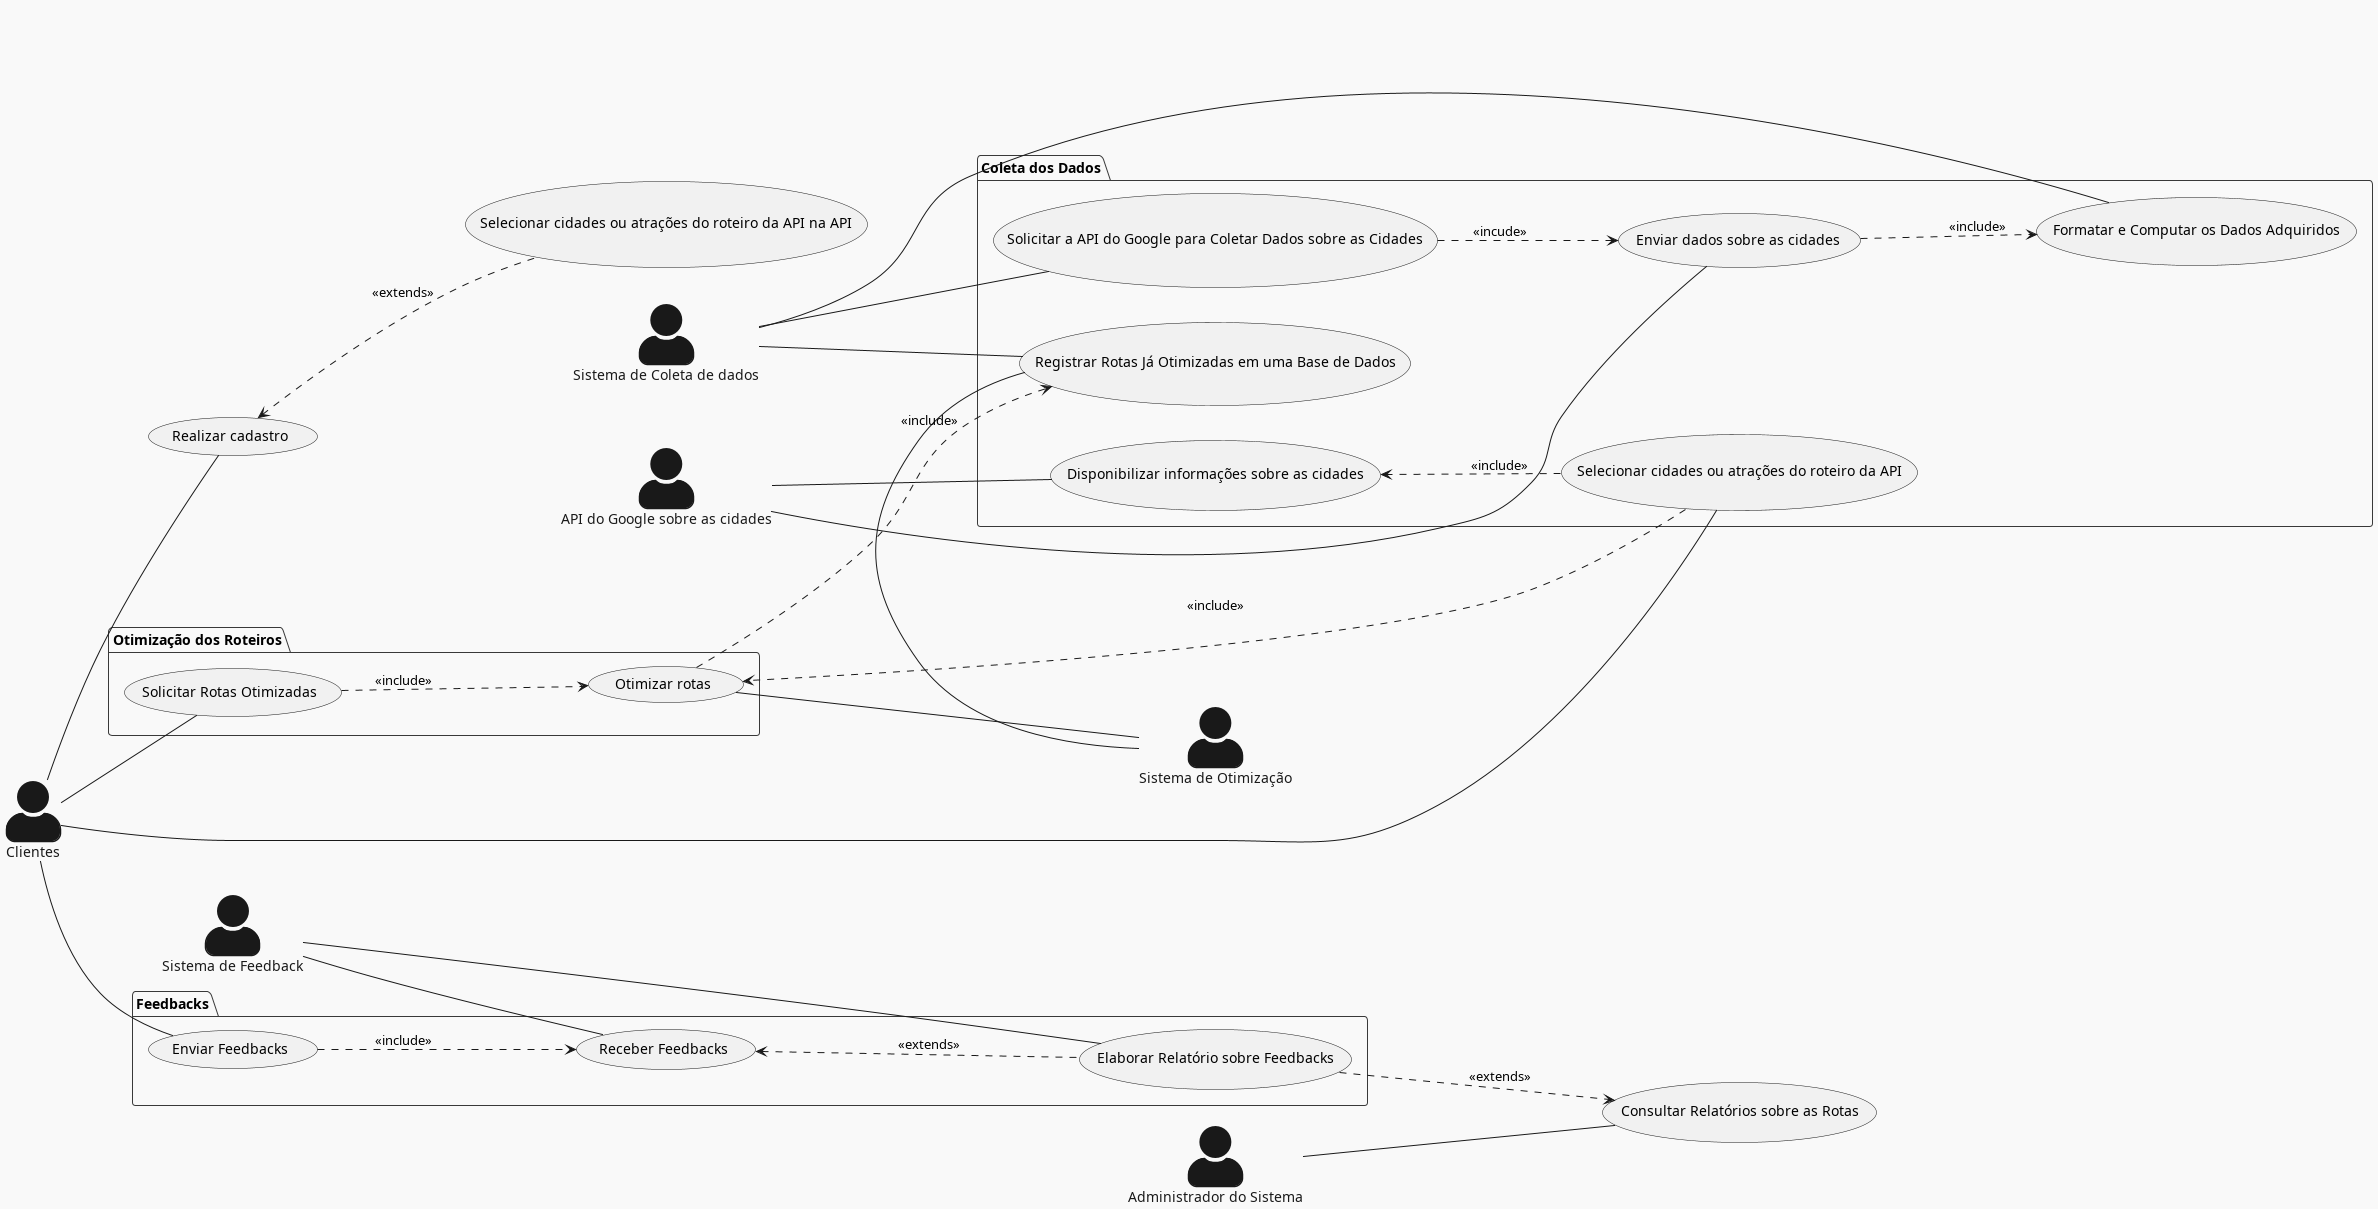
\includegraphics[scale=0.22]{Diagramas/DCU.png}\\
    \caption*{Fonte: Elaborado pelos autores}
\end{figure}

No diagrama de caso de uso, então, são observadas as interações entre os atores e as funcionalidades oferecidas pelo sistema de otimização de roteiros turísticos. O ator principal é denominado "Clientes", o qual interage com o sistema de diversas maneiras. Inicialmente, os clientes têm a capacidade de efetuar o cadastro no sistema, fornecendo suas informações pessoais para obter acesso às funcionalidades oferecidas.

Outra interação relevante é a capacidade dos clientes de "Enviar Feedbacks". Essa funcionalidade possibilita que os clientes forneçam suas opiniões, sugestões e avaliações sobre os roteiros turísticos e a experiência geral com o sistema. Esses feedbacks são valiosos para a melhoria contínua do sistema e para atender melhor às necessidades dos clientes.

Além do ator "Clientes", o "Administrador do Sistema" também desempenha um papel no diagrama. Ele tem acesso à funcionalidade de "Consultar Relatórios sobre as Rotas", que permite ao administrador visualizar relatórios detalhados elaborados sobre as rotas turísticas otimizadas. Tais relatórios são essenciais para o monitoramento do desempenho do sistema, a identificação de tendências e a tomada de decisões estratégicas.

O pacote "Otimização dos Roteiros" é um elemento-chave no diagrama, no qual o "Sistema de Otimização" desempenha um papel central. Ele oferece a funcionalidade de "Otimizar Rotas", a qual consiste no processo de otimização dos itinerários turísticos com base nas informações coletadas sobre as cidades ou atrações selecionadas. Essa funcionalidade é a essência do sistema.

O pacote "Coleta dos Dados" envolve o "Sistema de Coleta de Dados" e a "API do Google sobre as cidades". Esses atores trabalham em conjunto para coletar e disponibilizar informações detalhadas sobre as cidades e atrações turísticas. O sistema solicita dados relevantes à API do Google, a qual fornece as informações necessárias para que o sistema possa selecionar as cidades e atrações que atendam às preferências dos clientes.

Por fim, o pacote "Feedbacks" é responsável por coletar e armazenar os feedbacks enviados pelos clientes. O "Sistema de Feedback" possui a funcionalidade de "Armazenar dados do Feedback", permitindo que os feedbacks enviados pelos clientes sejam registrados para análise e futuras melhorias. Ademais, o sistema elabora relatórios sobre esses feedbacks, fornecendo informações importantes para avaliar a satisfação dos clientes e a eficácia do sistema em atender às suas expectativas.

Essas interações e funcionalidades detalhadas no diagrama de caso de uso oferecem uma visão clara das principais características do sistema de otimização de roteiros turísticos, enfatizando a personalização dos itinerários e a coleta de feedbacks como aspectos fundamentais para aprimorar a experiência dos clientes e garantir a eficiência do sistema

\subsection{Diagrama de Fluxo de Dados}

O diagrama de fluxo de dados é uma poderosa ferramenta de modelagem que descreve como as informações fluem dentro de um sistema, identificando as entradas, processamentos e saídas de dados. Nesta seção, apresentaremos o diagrama de fluxo de dados em três níveis (0, 1 e 2) do sistema de otimização de roteiros turísticos. O objetivo é fornecer uma visão detalhada das diferentes camadas do sistema, desde o nível mais abstrato até o mais detalhado.

\subsubsection{Nivel 0}

No DFD nível 0, foi representado a direção dos fluxos de informações que entram e saem do sitema principal, relacionando-os com os seus respectivos autores, os quais foram mostrados na Figura \ref{fig:DCU} 
\begin{figure}[H]
    \centering
    \caption{Diagrama Fluxo de Dados - Nível 0}
    \label{fig:DFD0}
    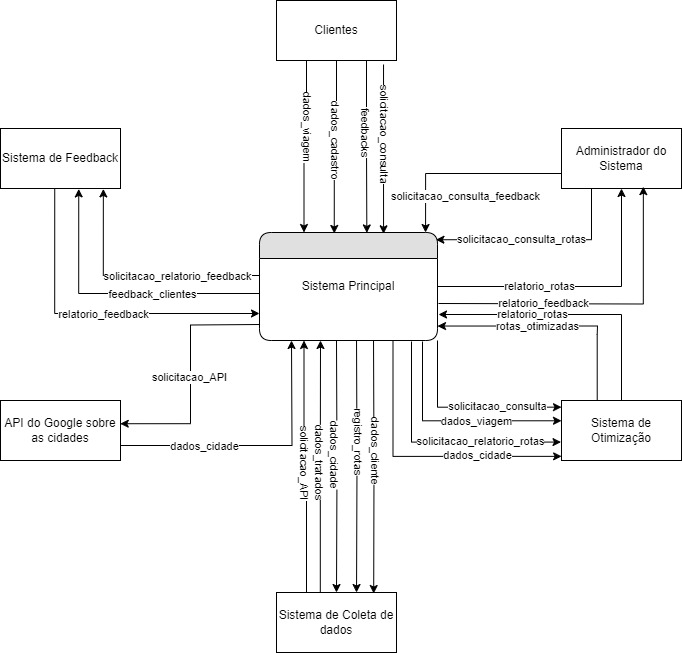
\includegraphics[scale=0.5]{Diagramas/DFD0.jpeg}\\
    \caption*{Fonte: Elaborado pelos autores}
\end{figure}

O sistema de otimização, por exemplo, envia para o sistema principal rotas otimizadas e recebe dados de cidades e solicitações de consulta. 


\subsubsection{Nivel 1}

Um Diagrama de Fluxo de Dados (DFD) de nível 1 é uma representação gráfica do sistema que descreve o fluxo de informações entre os principais processos e as principais entidades (ou atores) que interagem com o sistema.
No DFD de nível 1, o processo central do Diagrama de Contexto é decomposto em subprocessos menores, criando uma hierarquia de processos. Cada subprocesso representa uma parte específica do sistema e suas funcionalidades mais detalhadas. As setas representam os fluxos de dados entre os processos e as entidades, indicando a direção do fluxo das informações.

Esse nível de detalhamento torna o DFD de nível 1 mais compreensível e específico, permitindo que os analistas de sistemas e desenvolvedores tenham uma visão mais detalhada do funcionamento do sistema e das interações entre seus componentes.

Geralmente, em um DFD de nível 1, os processos principais são numerados, e as entradas e saídas de cada processo são identificadas por nome e direção do fluxo de dados. Isso ajuda a entender como as informações são processadas e compartilhadas entre os diferentes elementos do sistema.

\begin{figure}[H]
    \centering
    \caption{Diagrama Fluxo de Dados - Nível 1}
    \label{fig:DFD1}
    
\includegraphics[scale=0.5]{Diagramas/DFD1.png}\\
    \caption*{Fonte: Elaborado pelos autores}
\end{figure}

As relações são representadas da mesma maneira que no diagrama de nível 0. Aqui, porém, estão representadas também as bases de dados que são necssárias para que o sistema funcione e como os dados fluem entre elas e os processos. No caso, elas estão representadas por duas linhas paralelas com o nome da base entre as linhas


\subsubsection{Nivel 2}

O Diagrama de Fluxo de Dados de nível 2 para o processo de otimização de rota oferece uma visão mais detalhada e aprofundada do funcionamento interno desse processo crucial do sistema. Esse diagrama mostra como as informações fluem e são processadas dentro do sistema durante a etapa de otimização de roteiros turísticos.

O processo de otimização de rota é considerado o coração do sistema devido à sua importância estratégica e impacto direto na qualidade das experiências turísticas oferecidas aos clientes.  Na figura \ref{fig:DFD2} podemos visualizar esse diagrama:

\begin{figure}[H]
    \centering
    \caption{Diagrama Fluxo de Dados - Nível 2}
    \label{fig:DFD2}
    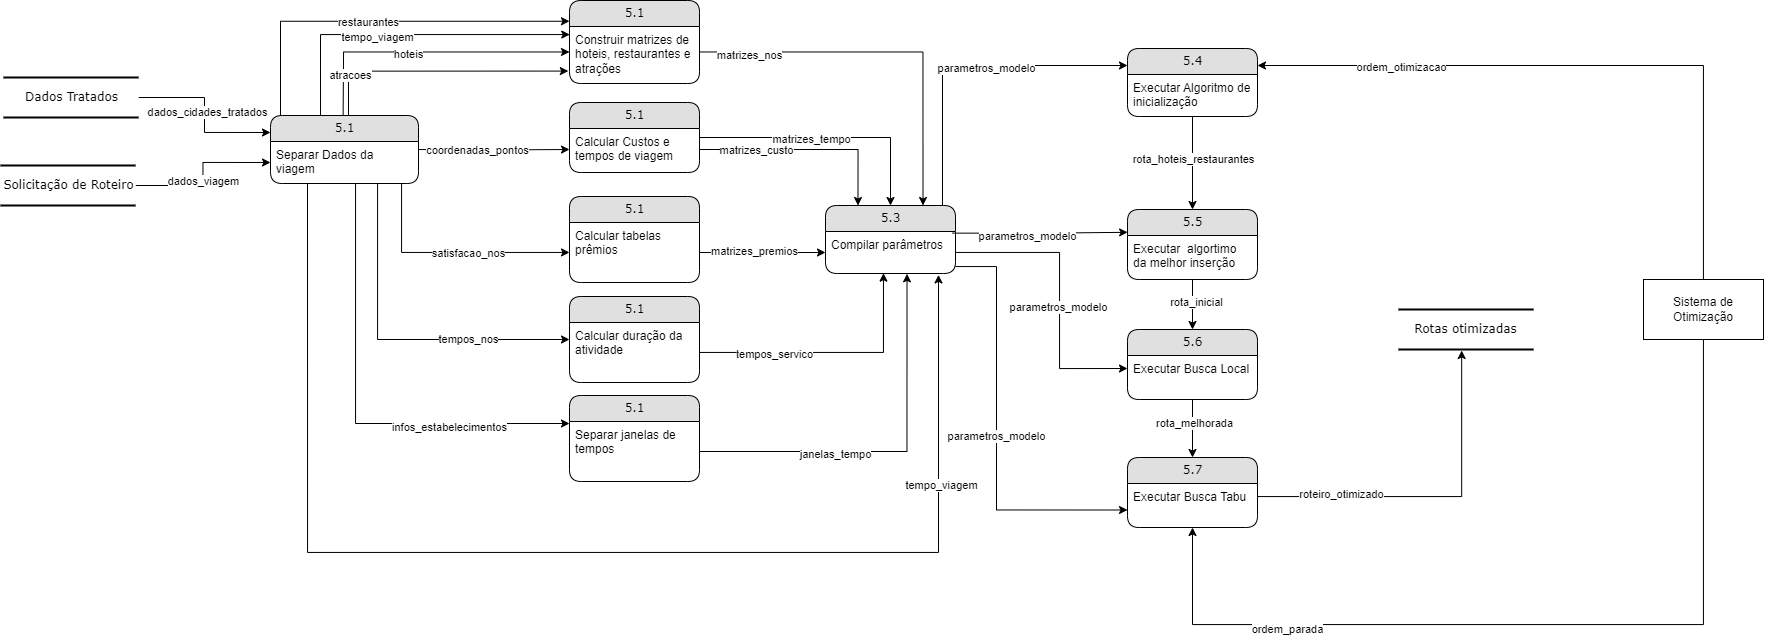
\includegraphics[scale=0.29]{Diagramas/DFD2.png}\\
    \caption*{Fonte: Elaborado pelos autores}
\end{figure}

A seguir, serão destacados os principais aspectos do Diagrama de Fluxo de Dados de nível 2 e sua relevância para o sistema:

    \textbf{Entradas Detalhadas:} O diagrama apresenta as entradas detalhadas necessárias para o processo de otimização de rota. Isso inclui informações sobre as preferências dos clientes, como as cidades ou atrações que desejam visitar, as restrições temporais e orçamentárias, entre outros dados relevantes, sobretudo, os parâmetros do modelod e otimização. Essas entradas são fundamentais para garantir que os roteiros sejam personalizados e adaptados às necessidades de cada turista.

    \textbf{Utilização de Modelos de Pesquisa Operacional:} O diagrama evidencia a aplicação dos modelos de Pesquisa Operacional no processo de otimização de rota. Esses modelos matemáticos avançados permitem resolver problemas complexos de forma eficiente, considerando restrições como janelas de tempo, custos e distâncias percorridas. A utilização desses modelos é essencial para garantir a criação de itinerários lógicos e otimizados.

    \textbf{Integração com o Sistema de Coleta de Dados:} O diagrama mostra como o processo de otimização de rota se integra com o Sistema de Coleta de Dados. Esse sistema é responsável por coletar informações detalhadas sobre as cidades e atrações turísticas, como horários de funcionamento, atrações disponíveis e dados relevantes. Esses dados são cruciais para a tomada de decisões durante a etapa de otimização.

    \textbf{Processamento e Geração de Rotas Otimizadas:} O diagrama revela como as informações coletadas e as entradas dos clientes são processadas para gerar rotas otimizadas. Nessa etapa, os algoritmos de Pesquisa Operacional são aplicados para calcular as melhores sequências de visitas, considerando as preferências dos clientes e as restrições das atrações. Esse processamento é o cerne do sistema, pois é responsável por criar os itinerários altamente satisfatórios para os turistas.

    \textbf{Saída de Rotas Otimizadas:} O diagrama destaca a saída resultante do processo de otimização, ou seja, as rotas turísticas otimizadas. Essas rotas representam os itinerários personalizados para cada cliente, levando em conta suas preferências e as características das atrações turísticas. Essa saída é o produto final do processo e será utilizada para guiar os turistas em suas jornadas.

O processo de otimização de rota é o coração do sistema porque é o ponto central onde ocorre a tomada de decisões fundamentais para a satisfação dos clientes. Através da aplicação de algoritmos avançados e integração de informações relevantes, esse processo é responsável por criar os itinerários personalizados e eficientes que maximizam a experiência do viajante.

\subsection{Diagrama de Entidade Relacionamento}

\begin{figure}[H]
    \centering
    \caption{Diagrama de Entidade Relacionamento}
    \label{fig:DER}
    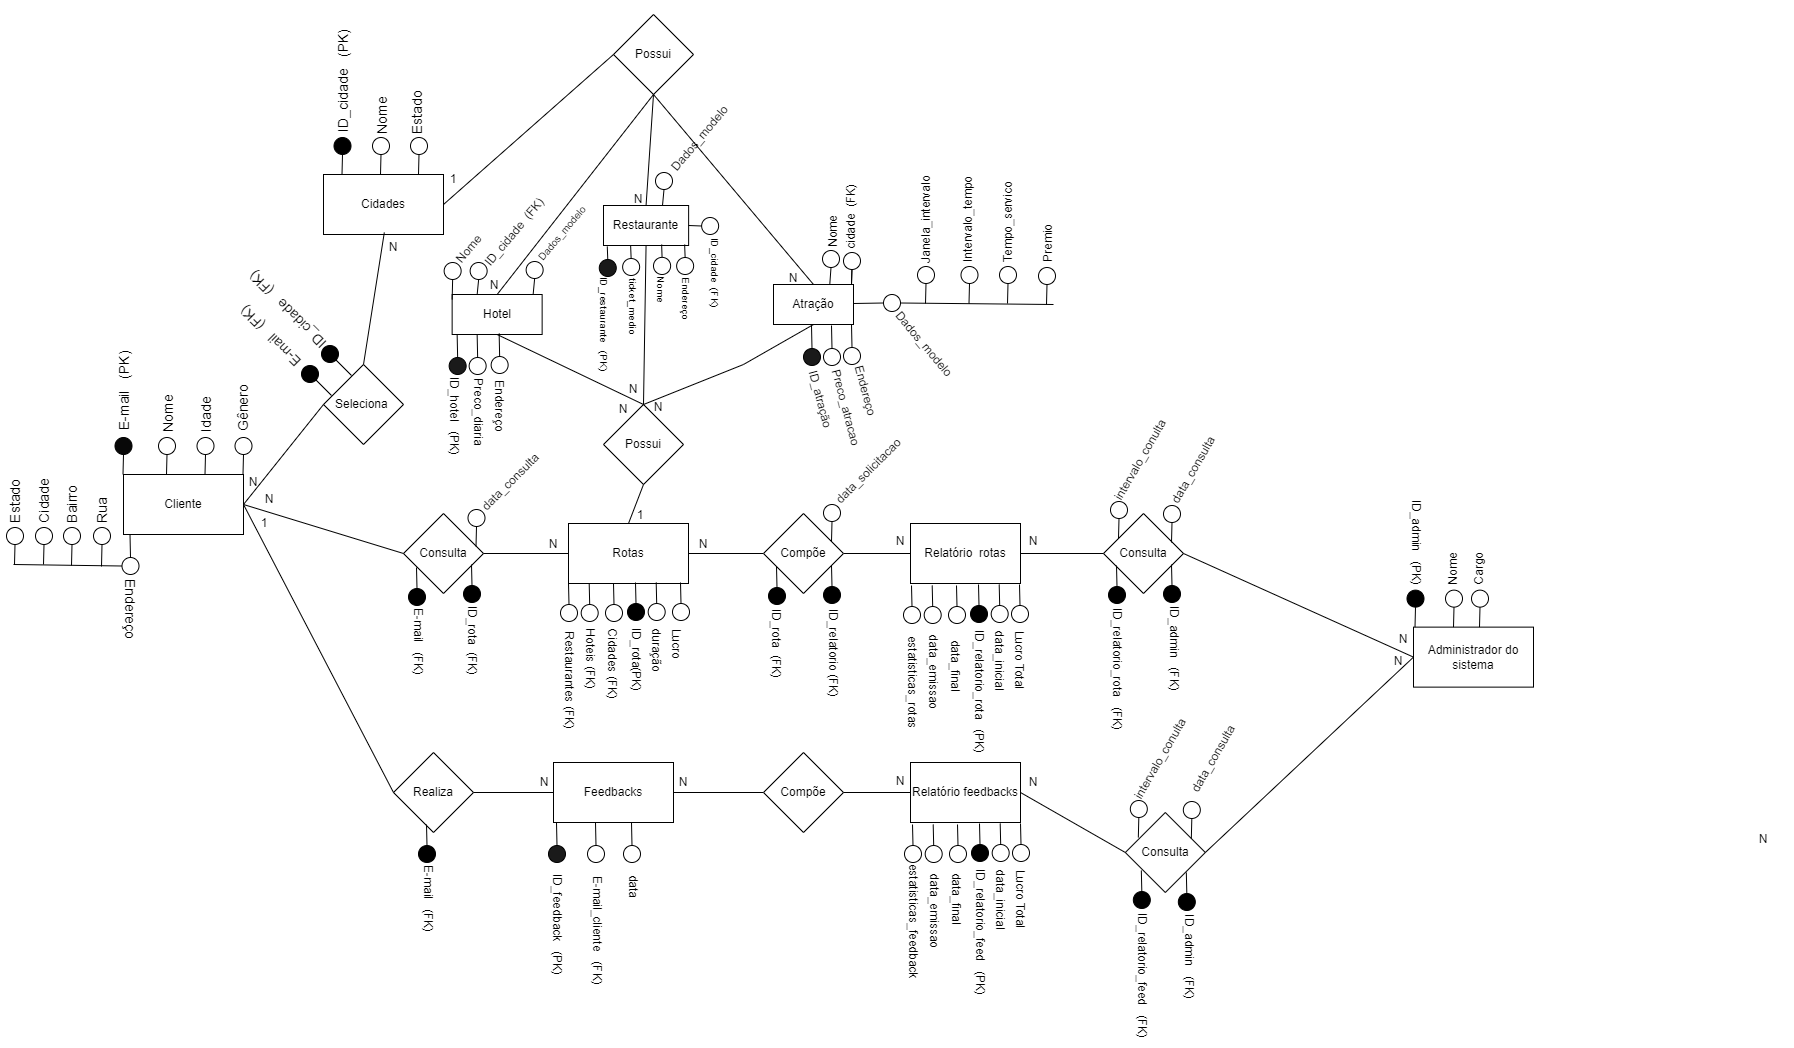
\includegraphics[scale=0.3]{Diagramas/DER.png}\\
    \caption*{Fonte: Elaborado pelos autores}
\end{figure}

O diagrama busca fornecer informações sobre como as entidades se relacionam dentro do sistema. A entidade "cliente" seleciona a entidade "Cidades" e essa seleção possui os atributos do email do cliente e do ID das cidades. Como um cliente pode selecionar várias cidades e uma cidade pode ser selecionaada por vários clientes, a relação construída é de "N para N". 

Outros aspectos que podem ser percebidos no diagrama é que rotas podem ser consultadas por clientes em alguma data e possuem Hoteis, atrações e Restaurantes. Estes, por sua vez, são "possuídos" (ou seja, pertencem) por uma cidade. Neste último caso, temos uma relação de "1 para N", porque uma cidade pode possuir várias dessas entidades, mas elas pertencem a uma, e somente uma, cidade. 

As demais relações podem ser entendidas e explicadas por vias análogas e a relação entre elas visualizada de maneira mais simples no modelo relacional. 



\subsection{Modelo Relacional}


\begin{figure}[H]
    \centering
    \caption{Modelo relacional}
    \label{fig:DER}
    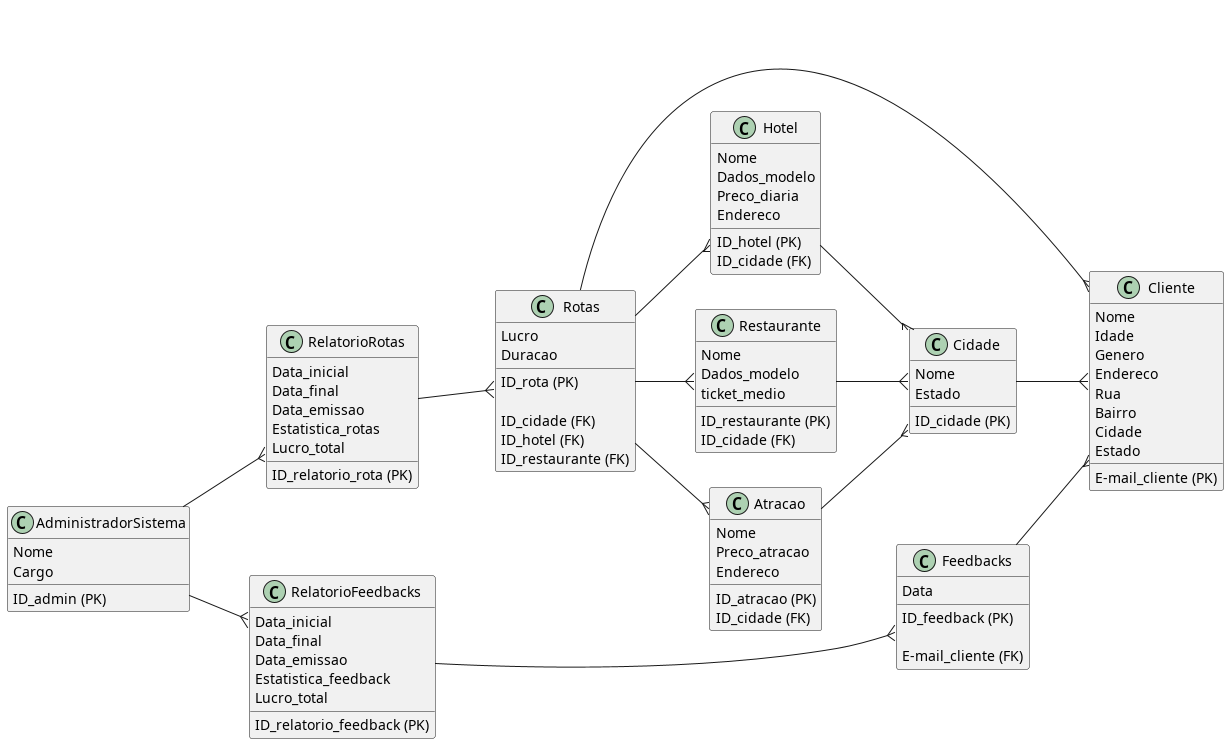
\includegraphics[scale=0.42]{Diagramas/Relacional.png}\\
    \caption*{Fonte: Elaborado pelos autores}
\end{figure}

O modelo relacional apresentado descreve a estrutura de dados do sistema de otimização de roteiros turísticos em PlantUML. Nesse modelo, temos diversas classes que representam as principais entidades do sistema, suas atribuições e relacionamentos entre si.

As classes principais incluem:
\begin{enumerate}
    \item \textbf{Cliente}: Representa os clientes do sistema e suas informações pessoais, como e-mail, nome, idade, gênero e endereço.
    \item \textbf{Cidade}: Refere-se às cidades cadastradas no sistema, com atributos como ID da cidade, nome e estado.
    \item \textbf{Hotel}: Descreve os hotéis disponíveis nas cidades do sistema, com informações como ID do hotel, nome, ID da cidade, dados do modelo, preço da diária e endereço.
    \item \textbf{Restaurante}: Representa os restaurantes presentes nas cidades, com atributos como ID do restaurante, nome, ID da cidade, dados do modelo e ticket médio.
    \item \textbf{Atração}: Refere-se às atrações turísticas nas cidades, com atributos como ID da atração, nome, ID da cidade, preço da atração e endereço.
    \item \textbf{Rotas}: Representa as rotas turísticas criadas pelo sistema, com informações como ID da rota, ID da cidade, ID do hotel, ID do restaurante, lucro e duração.
    \item \textbf{RelatorioRotas}: Descreve os relatórios gerados para as rotas, contendo ID do relatório, data inicial, data final, data de emissão, estatísticas das rotas e lucro total.
    \item \textbf{Feedbacks}: Representa os feedbacks enviados pelos clientes, com atributos como ID do feedback, e-mail do cliente e data do feedback.
    \item \textbf{RelatorioFeedbacks}: Descreve os relatórios gerados para os feedbacks, contendo ID do relatório, data inicial, data final, data de emissão, estatísticas dos feedbacks e lucro total.
    \item \textbf{AdministradorSistema}: Refere-se aos administradores do sistema, com informações como ID do administrador, nome e cargo.
\end{enumerate}

Os relacionamentos entre as classes são representados por associações. Por exemplo:
\begin{itemize}
    \item \textbf{Cliente} está associado à \textbf{Cidade}, \textbf{Rotas} e \textbf{Feedbacks}, indicando que um cliente pode estar relacionado a várias cidades, rotas e feedbacks.
    \item \textbf{Cidade} possui associações com \textbf{Hotel}, \textbf{Restaurante} e \textbf{Atração}, mostrando que uma cidade pode ter vários hotéis, restaurantes e atrações associados a ela.
    \item \textbf{Rotas} está associado a \textbf{Hotel}, \textbf{Atração} e \textbf{Restaurante}, indicando que uma rota pode incluir vários hotéis, atrações e restaurantes.
    \item \textbf{RelatorioRotas} está associado a \textbf{Rotas}, significando que um relatório de rotas pode abranger várias rotas.
    \item \textbf{RelatorioFeedbacks} está associado a \textbf{Feedbacks}, indicando que um relatório de feedbacks pode conter vários feedbacks.
    \item \textbf{AdministradorSistema} está associado a \textbf{RelatorioRotas} e \textbf{RelatorioFeedbacks}, mostrando que um administrador pode ter acesso a vários relatórios de rotas e feedbacks.
\end{itemize}

Esse modelo relacional descreve a estrutura de dados do sistema e os relacionamentos entre as entidades, fornecendo uma base sólida para a implementação do sistema de otimização de roteiros turísticos. Ele permite uma organização eficiente e precisa das informações, facilitando a consulta e manipulação dos dados, bem como a geração de relatórios para auxiliar a tomada de decisões.



\section{Referências}
GONÇALVES, V. A.; REIS, D. M. dos; MAIA, E. H. B.; BEIRIGO, B. A.; SOUZA, S. R. de; BARRIENTOS, A. Y. M. ALGORITMO GENÉTICO BASEADO EM CHAVES ALEATÓRIAS PARA O ORIENTEERING PROBLEM WITH TIME WINDOWS. Revista Interdisciplinar de Pesquisa em Engenharia, [S. l.], v. 2, n. 10, p. 90–104, 2017. DOI: 10.26512/ripe.v2i10.21730. Disponível em: https://periodicos.unb.br/index.php/ripe/article/view/21730. Acesso em: 4 jul. 2022.

TURISMO perde US\$ 2 trilhões em 2021 por causa da pandemia BR. ONU news, [S. l.], p. 1-1, 21 nov. 2021. Disponível em: 29/11/2021. Acesso em: 8 ago. 2022.
REVER totalmente o turismo global pode representar uma oportunidade no pós-pandemiaBR. ONU news, [S. l.], p. 1-1, 9 jan. 2022. Disponível em: 09/01/2022. Acesso em: 8 ago. 2022.

SILVA, Admilson Alcântara; MORABITO, Reinaldo; PUREZA, VItória. Optimization approaches to support the planning and analysis of travel itineraries. Expert System with Applications, [s. l.], v. 112, 1 dez. 2018. Disponível em: 1/12/2018. Acesso em: 8 ago. 2022.

\end{document}